%%%%%%%% ICML 2023 EXAMPLE LATEX SUBMISSION FILE %%%%%%%%%%%%%%%%%

\documentclass{article}

% Recommended, but optional, packages for figures and better typesetting:
\usepackage{microtype}
\usepackage{graphicx}
\usepackage{subfigure}
\usepackage{booktabs} % for professional tables
\newcommand{\tz}[1]{{\color{magenta}TZ: #1}}
\newcommand{\jh}[1]{{\;\color{red}JH: #1}}
\newcommand{\bc}[1]{{\color{olive}BC: #1}}

% hyperref makes hyperlinks in the resulting PDF.
% If your build breaks (sometimes temporarily if a hyperlink spans a page)
% please comment out the following usepackage line and replace
% \usepackage{icml2023} with \usepackage[nohyperref]{icml2023} above.
\usepackage{hyperref}


% Attempt to make hyperref and algorithmic work together better:
\newcommand{\theHalgorithm}{\arabic{algorithm}}

% Use the following line for the initial blind version submitted for review:
\usepackage{icml2023}

% If accepted, instead use the following line for the camera-ready submission:
% \usepackage[accepted]{icml2023}

% For theorems and such
\usepackage{amsmath}
\usepackage{amssymb}
\usepackage{mathtools}
\usepackage{amsthm}

% if you use cleveref..
\usepackage[capitalize,noabbrev]{cleveref}

%%%%%%%%%%%%%%%%%%%%%%%%%%%%%%%%
% THEOREMS
%%%%%%%%%%%%%%%%%%%%%%%%%%%%%%%%
\theoremstyle{plain}
\newtheorem{theorem}{Theorem}[section]
\newtheorem{proposition}[theorem]{Proposition}
\newtheorem{lemma}[theorem]{Lemma}
\newtheorem{corollary}[theorem]{Corollary}
\theoremstyle{definition}
\newtheorem{definition}[theorem]{Definition}
\newtheorem{assumption}[theorem]{Assumption}
\theoremstyle{remark}
\newtheorem{remark}[theorem]{Remark}

% Todonotes is useful during development; simply uncomment the next line
%    and comment out the line below the next line to turn off comments
%\usepackage[disable,textsize=tiny]{todonotes}
\usepackage[textsize=tiny]{todonotes}


% The \icmltitle you define below is probably too long as a header.
% Therefore, a short form for the running title is supplied here:
\icmltitlerunning{Submission and Formatting Instructions for ICML 2023}

\begin{document}

\twocolumn[
% \icmltitle{The Anna Karenina Conjecture of Intelligence}
% \icmltitle{The Intelligence Bottleneck}
\icmltitle{The Scaling Law of Representational Convergence}

% It is OKAY to include author information, even for blind
% submissions: the style file will automatically remove it for you
% unless you've provided the [accepted] option to the icml2023
% package.

% List of affiliations: The first argument should be a (short)
% identifier you will use later to specify author affiliations
% Academic affiliations should list Department, University, City, Region, Country
% Industry affiliations should list Company, City, Region, Country

% You can specify symbols, otherwise they are numbered in order.
% Ideally, you should not use this facility. Affiliations will be numbered
% in order of appearance and this is the preferred way.
\icmlsetsymbol{equal}{*}

\begin{icmlauthorlist}
\icmlauthor{Firstname1 Lastname1}{equal,yyy}
\icmlauthor{Firstname2 Lastname2}{equal,yyy,comp}
\icmlauthor{Firstname3 Lastname3}{comp}
\icmlauthor{Firstname4 Lastname4}{sch}
\icmlauthor{Firstname5 Lastname5}{yyy}
\icmlauthor{Firstname6 Lastname6}{sch,yyy,comp}
\icmlauthor{Firstname7 Lastname7}{comp}
%\icmlauthor{}{sch}
\icmlauthor{Firstname8 Lastname8}{sch}
\icmlauthor{Firstname8 Lastname8}{yyy,comp}
%\icmlauthor{}{sch}
%\icmlauthor{}{sch}
\end{icmlauthorlist}

\icmlaffiliation{yyy}{Department of XXX, University of YYY, Location, Country}
\icmlaffiliation{comp}{Company Name, Location, Country}
\icmlaffiliation{sch}{School of ZZZ, Institute of WWW, Location, Country}

\icmlcorrespondingauthor{Firstname1 Lastname1}{first1.last1@xxx.edu}
\icmlcorrespondingauthor{Firstname2 Lastname2}{first2.last2@www.uk}

% You may provide any keywords that you
% find helpful for describing your paper; these are used to populate
% the "keywords" metadata in the PDF but will not be shown in the document
\icmlkeywords{Machine Learning, ICML}

\vskip 0.3in
]

% this must go after the closing bracket ] following \twocolumn[ ...

% This command actually creates the footnote in the first column
% listing the affiliations and the copyright notice.
% The command takes one argument, which is text to display at the start of the footnote.
% The \icmlEqualContribution command is standard text for equal contribution.
% Remove it (just {}) if you do not need this facility.

%\printAffiliationsAndNotice{}  % leave blank if no need to mention equal contribution
\printAffiliationsAndNotice{\icmlEqualContribution} % otherwise use the standard text.

% \title{The Anna Karenina Conjecture of Intelligence}
% \date{April 2023}


\section{Introduction}

\jh{Todo: Anna Karenina -> Intelligence bottleneck, give full credit to Boaz Barak.}
\jh{Add experiments: meta-plot in the alignment of methods to the human brain. Jim's work.}
\jh{Add data from Dreamsim: larger models are closerly aligned with humans.}
\jh{BAPPS, DREAMSIM, BRAINSCORE, THINGS}
\jh{Alignment of models to models}
\jh{MS-COCO brainscores like dataset?}
\jh{Alignment of vision to LLMs: can we just annotate vision scores}
\jh{Figure 1/2 illustrates there is 1 universal: Phillip}
\jh{Figure 3: VISION (JACOB)}
\jh{Figure 4: LLM (BRIAN)}
\jh{FIgure 5: Generalization bounds.}
\jh{UCE style for cross model convergence}
\jh{to cite  and all read: https://www.biorxiv.org/content/10.1101/2022.03.28.485868v2.full.pdf}

In biology, when two species are subjected to similar selective pressures, they may develop similar traits, despite sharing no genetic lineage~\cite{XX}. This is called convergent evolution. The same can be true in artificial systems~\cite{XX}.

We conjecture that this is what is happening in the current development of AI. Different AI systems developed by different groups are all subject to similar pressures, and these pressures are causing a narrowing of the algorithmic landscape. While this may be a bad thing, reducing the diversity of research might also be inevitable, and that's what we will argue. We further conjecture that this convergence is shared between all systems that approach human-level intelligence in universes like our own. Humans, aliens, and AIs alike will all develop similar cognitive competences \textit{and} mechanisms.

Our basic argument goes as follows: 
\begin{enumerate}
\item The more competencies we require of a system, the fewer systems satisfy all these competencies.
\item Human-like intelligence is characterized by its generality. It requires lots of competencies.
\end{enumerate}

All intelligent systems are alike, but every unintelligent system is unintelligent in its own way.

%All performant and efficient systems are alike, and every other system is either not performant or not efficient.

We see this convergence anywhere selective pressure is increased. At a high school high jump competition, there are many body types, many different jumping styles, many types of shoes, etc. At the Olympics, all the high jumpers are tall and skinny, perform the Fosbury flop, and wear lightweight shoes with spikes.

This fact, a tautology really, is generally called the ``Anna Karenina Principle.''~\cite{XX} While it is apparent from first principles, the degree to which it holds explanatory power varies from field to field and depends on the degree of selective pressure. We argue that AI is a field where this principle can indeed explain a lot. The rest of this paper is a meta-scientific investigation of the many ways convergence is playing out in AI. The \textit{conjecture} part of our argument is that Anna Karenina explains the convergences we are seeing and that these trends will continue.

\begin{figure}[t]
    \centering
    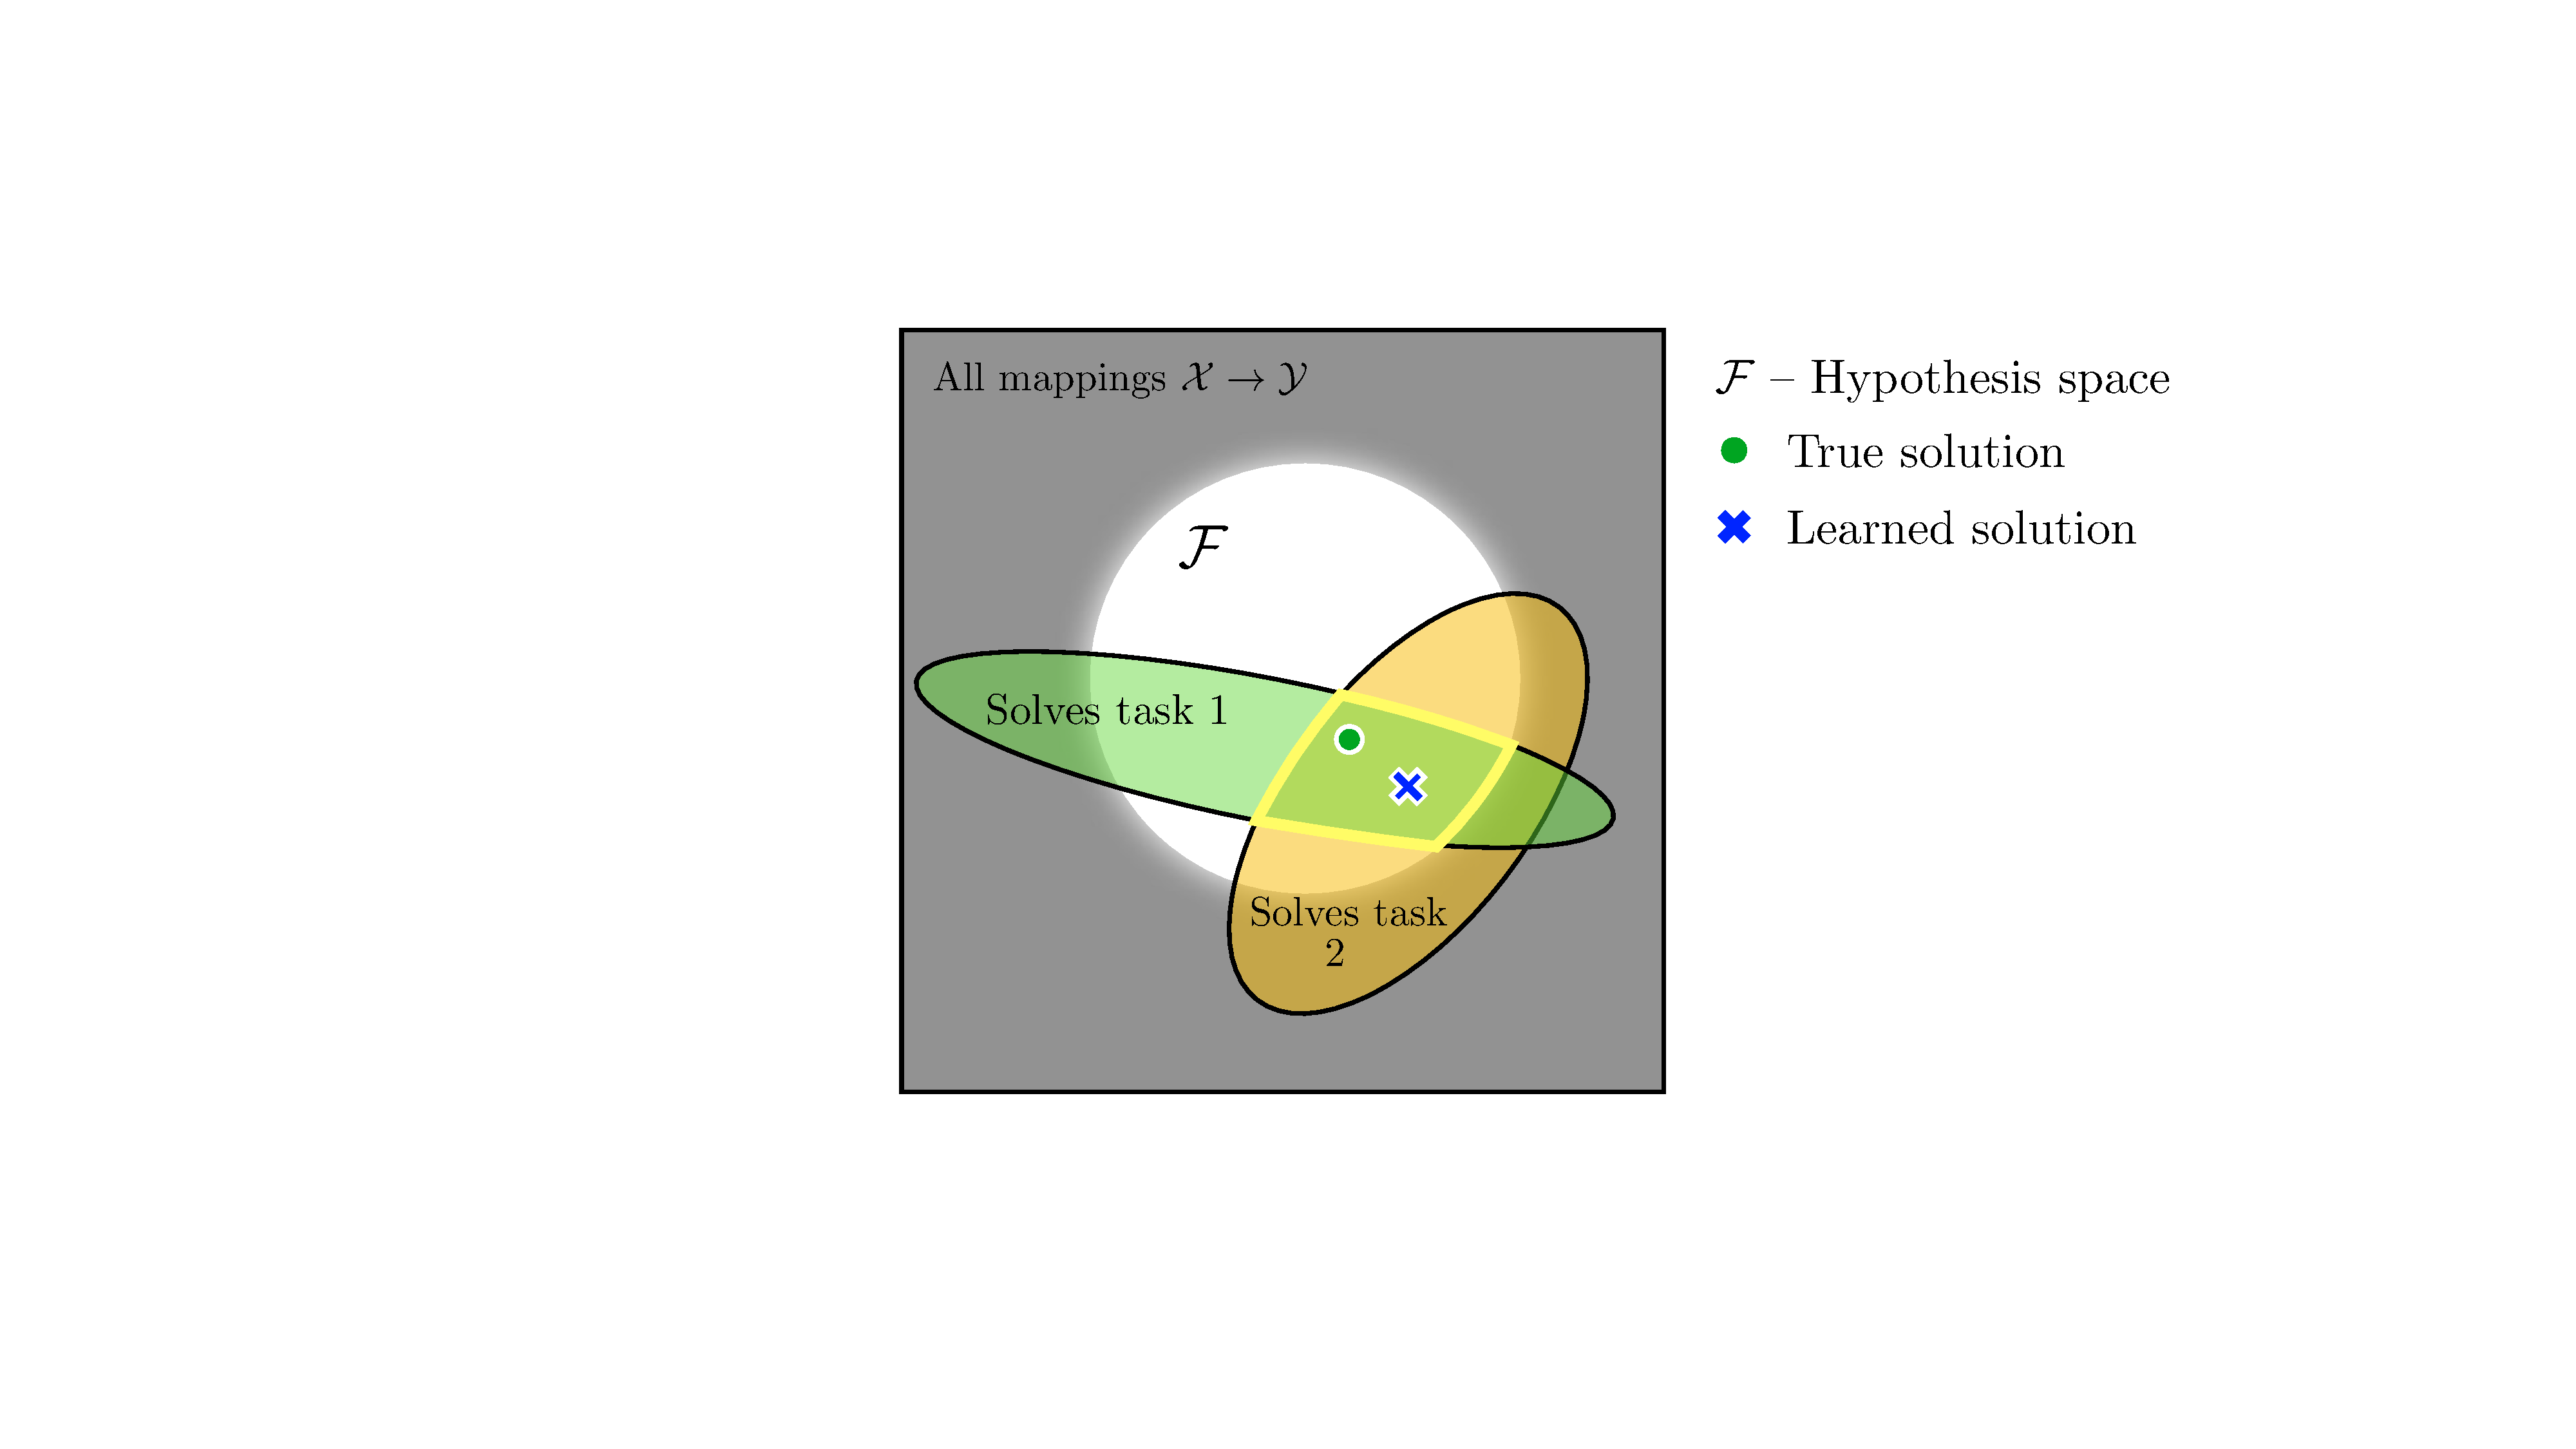
\includegraphics[width=1.0\linewidth]{figures/tasks_are_constraints.pdf}
    \caption{Tasks are constraints. More tasks, fewer solutions to all of them.}
\end{figure}

Even if it is true that all systems, subject to the same pressures, eventually converge, it remains a question as to when they converge. \jh{what does it even mean to converge, or are they are always converging? Does it ever diverge? Would divergent evolution to 2 extreme niches considered divergent? or convergent because they have settled at a steady state?} When are the pressures sufficiently similar? In some ecosystems, there are many niches, each with its own pressures. Then we should expect a diversity of species. In other ecosystems, there might be just a single niche. We call this latter setting the Anna Karenina regime. We will argue that perception is now in an Anna Karenina regime, and so is generation. However, other aspects of intelligent agents might not be, including morphology, action, reasoning, etc.

Once in the Anna Karenina regime, the bitter lesson takes hold. You are in a convergent basin where just ``scaling up'' leads you ever closer to the minimum.

\bc{Two statements can be made after this:
1) a hedge of saying it could still be a local minimum and a drastic change in the field must occur to change the trajectory of that minimum is necessary.
2) Definitively declare that this is a global minimum.
I prefer 1}

\section{Defining Intelligence}
As AI systems become more capable, they are increasingly subjected to the selective pressure of needing to achieve goals and perform tasks in various real-world environments. Systems that are too narrowly specialized will fail or be limited. Just as convergent evolution leads biological species to develop similar adaptive traits when facing similar environmental pressures, the pressure for general intelligence is causing different AI systems to develop similar underlying competencies and mechanisms.

 As AI systems aim to develop human-level intelligence, defined by its generality across environments, they need to develop learning and adaptation abilities to achieve goals across many contexts flexibly. This pressure towards general competency is nudging different AI architectures in similar directions, leading to convergence. 
 
 % If we define intelligence as the ability to achieve goals across environments \cite{legg2008machine}, then the evolutionary pressure on AI systems to develop versatile, general capabilities can explain why continued advances in AI may lead to convergence, as this pressure shapes the emergence of the competencies and mechanisms needed for broad, human-like intelligence.

 If we adopt the definition of intelligence as the ability to achieve goals in various environments~\cite{legg2008machine}, then the evolutionary pressures on AI systems to develop versatile and general capabilities provide a plausible explanation for the ongoing convergence in AI advancements. These pressures are likely to guide the development of competencies and mechanisms necessary for achieving broad, human-like intelligence.
 
\section{Convergence \#1: models and minds} \label{sec:models-and-minds}

The human brain has five canonical modalities to experience the world. These sensory modalities are the only functional inputs of the external world to the brain. With the rapid development and distribution of the computer screen, the sense of vision has become the dominant modality in which we organize and communicate our knowledge due to its scalability. Capable of being recorded, replicated, and transmitted over large distances makes vision noticeably more efficient to distribute throughout human ecosystems than the other senses. Furthermore, considering that about thirty percent of the primate brain is dedicated to visual processing, it makes sense as the modality of choice for studying the inputs to intelligence.

From this perspective, it may not be as surprising that the vision modality became one of the earliest successes for the development of compelling artificial intelligence models that rely on adapting to large volumes of data \cite{krizhevsky2017imagenet, russakovsky2015imagenet}. And as a reflection of the amount of biological relevance present in this data, the representations that emerge in these artificial models are similar to those in human and animal brains. We conjecture that the models are trained on similar data and tasks as humans were trained/evolved on \cite{yamins2014performance}. More recently, the similarities have expanded beyond visual perception; artificial models have had significant success in abstractions beyond the sensory input, such as language \cite{schrimpf2021neural, zhang2019bertscore}.

This commonality between artificial models and biological systems likely stems from the universal underpinnings of information processing. Even though the mediums may differ -- silicon transistors versus biological neurons --, the fundamental problem is the same: efficiently extracting and understanding the underlying structure in the data. The tasks that the human visual system has been honed to perform through evolution -- like segmentation, detection, and whole-image classification -- are also the ones that we find most beneficial for our artificial systems. This phenomenon provides a potent testament to the robustness and adaptability of computational principles and the possibility of reaching similar solutions to the same problems, regardless of the substrate in which the computation is performed.

LPIPS and perceptual alignment papers. In LPIPS we found that if you train a net on any of a variety of tasks -- supervised, self-supervised, etc -- it learns to measure distances in a way that correlates with how humans perceive perceptual similarity.

objective (and data) affect alignment \citep{muttenthaler2022human}
BERT features correlate w human \citep{zhang2019bertscore}

\bc{Not sure if this next paragraph fits in with the rest:}
The study of artificial intelligence has led to remarkable discoveries, particularly in visual perception and language processing. Interestingly, the evolutionary path of biological systems and our artificial technology have resulted in striking similarities, despite their vastly divergent developmental trajectories. For instance, artificial models optimized for mapping visual percepts to language (e.g. segmentation, detection, whole-image classification) all appear to reach a common solution. Stepping back, the task space between these mappings may also be converging when you consider the scope of broader datasets. Segmentation, detection, and whole-image classification are problems with differing spatial granularity.

\section{Convergence \#2: models and physics}

% Generative models learn latent representations that act like graphics primitives -- lights, camera angle, consistent geometry, etc. We conjecture that this is because both are models of physics, and lights, cameras, and geometry are ``true'' properties of the physical world. All reasonable models will converge on these truths.

Physical laws govern our world. These laws are not initially known by humans, but some have been gradually discovered over thousands of years. Since ancient times, philosophers and scientists have come up with hypotheses that potentially explain certain observed phenomena (such as the rise and the fall of the sun), gather new data in experiments to verify or falsify their hypotheses, and eventually converge on certain explanations (such as the rotation of the earth) \citep{newton1989truth}. To explain the observed phenomenon, we developed an understanding of something that is not (as easily and directly) observable. These observations are distilled into abstractions, which are promoted to the level of laws because they survive and remain consistent after repeated counterfactual and adversarial testing.
\jh{Is there a compression argument here? The minimal length description of the observations is the physical laws that governs them. Any description that is smaller is either wrong or identical, and the previous description was verbose.}


Similar to humans, certain artificial models also explain certain observations of the real world. Through a similar process of repeated testing in the optimization and compression, artificial models must also develop abstractions of their observations. Generative neural networks are artificial models trained to \emph{model} a certain part of the real world, \textit{e.g.}, 2D photos of objects. After training on a dataset of samples, without supervision on how the world works, they can be used to generate synthetic 2D images that look just like a real photo, 
% or short stories that read like they are from human writers, 
or even effective chemical molecules. Such models have displayed a strong capability to produce believable samples, but do they really understand the data they are approximating? Do artificial models understand the optical process that governs how a photo is captured? Do they understand the chemical reactions among different molecules? The answer, we argue, is \emph{yes}. While current artificial systems do not perform their experimentation or counterfactuals, their learning operates under the same constraints as the abstractions and physical laws we develop. Namely, every representation generated (i.e., abstraction) by the model must fit as many observations as possible (i.e., have high fitness). Optimization processes like stochastic gradient descent act as the repeated testing that their representations are subjected to. But without the agency of creating its own counterfactuals, this learning has the limitation of only being able to explain existing observations. Though as these models interact more with the real world in a more autonomous fashion, a growing fraction of the observations they learn from will be from their own actions.

\bc{This paragraph needs citations}
When fit to 2D images, generative models have shown an emergent understanding of the 3D structures, light transport, or temporal effects of the underlying physical world, even though they are never trained on these structures. In particular, such models disentangles properties like \emph{3D rotation angle}, \emph{object size}, and \emph{color} as controllable knobs \citep{jahanian2019steerability}. For a generated image of an object, one can tune these knobs to \emph{independently} control the corresponding properties. In other words, by just learning to generate 2D images, the model develops an understanding of the underlying physical structures. 


\tz{
identifiability?
}

\section{Convergence \#3: models and models}

The alignment of model and human representation, as revealed empirically, raises the question of whether models themselves are converging. Architecturally, this convergence has been apparent. Innovations such as residual connections, weight-reuse, attention mechanisms, and transformers being universally adopted across various tasks and sensory modalities. 
Such generalist architecture components have proven to yield little to no performance loss over their specialist counterparts. They are increasingly adopted over the machine learning community due to their capability, versatility, and usefulness in multi-task multi-modal models. While these are likely not at the very ``optimality'', the ongoing convergence to such general-purpose architectures components is evident.


Another critical aspect of convergence has emerged in the form of representational convergence. Here, representational convergence pertains to the concept that models progressively align toward the same functional characterization of the data. We discuss several threads on the topic of representational convergence.
Note, we are not concerned with how we have arrived at the same representation or whether these models have learned the same mechanistic decision processes. Indeed, it's essential to acknowledge that not every domain within the field has undergone through this ``representational convergence'', a topic we will delve into subsequently.


\bc{Though "All roads lead to Rome" is a common phrase, maybe we should cite https://arxiv.org/pdf/2106.07682.pdf which makes the same case with the same phrase}
\paragraph{Representational Convergence: Many Roads to Rome.}

In a deep neural network, input data is processed layer by layer. Therefore, we can look at network's \emph{representation} of some input data by extracting the intermediate activations (\emph{i.e.}, outputs of an intermediate layer). And we can compare different networks representation by comparing their intermediate activations. 
Recent works identified that such deep neural network models, even when trained with different architectures and/or different objectives and/or different dataset, can arrive at the same representation up to an affine transform \citep{moschella2022relative,klabunde2023similarity}. This might not be surprising. After all, we have established that different model representations converge to biological representations, and argued for this from the intelligence perspective, \emph{i.e.}, a ``necessity driven by intelligence'' \Cref{sec:models-and-minds}.  In this section, we take a machine learning perspective, and discuss how the very setting for learning these models (that is parametrizations, data, optimizations, etc.) can suggest such a convergence of different types models.

\jh{will revise. mostly just wrote down whatever came to mind}

\paragraph{Scaling Law: Solution Convergence from Big Data}
\jh{big models scale predictably with params. Bigger models require less and less fine-tuning.}
% The increasing prominence of deep learning models has drawn attecntion to the financial incentives associated with large models. 
% Scaling up models has become a central focus for those wishing to obtain performance regardless of efficiency of the algorithm itself. With the cost of amassing data and training these models continues to rise, there is a strong interest in understanding how models scale with parameters.

With more data points, the volume of representation that satisfies the data constraints must proportionately grow smaller. This has been previously termed as the Contravariance principle by~\cite{cao2021explanatory}, which states that the set of solutions to an easy goal is large, while the set of solutions to a challenging goal is comparatively smaller. In other words, the size of the set of optima or solutions is contravariant with the difficulty of the optimization problem. Hence, with increased scale of data, given the same algorithmic family (e.g., transformer trained with SGD), there must exist a predictive continuum of model's representational and generalizing capabilities.

This study of how models behave with scale is referred to as the scaling law. Scaling law studies a phenomena of how the model's for in- and out-of-domain generalization changes with data and parameter scale.
The first work can be dated back to~\cite{cortes1993learning}, which has been revisited by~\cite{hestness2017deep} for the modern deep learning era. Since then, the scaling law has emerged as a fundamental area of interest, leading to numerous follow-up studies that attempt to uncover the equation governing the scaling law through empirical measurements~\cite{rosenfeld2019constructive,kaplan2020scaling,hoffmann2022training}. So far there has not been any work demonstrating how to modify the exponent of the power law within the family of deep neural networks optimizing on natural data. Understanding the power law within the context of the scaling law remains an active area of research, with some initial studies investigating scaling laws in the context of kernels~\cite{bahri2021explaining}. 

The log-linear relationship between scale and model performance implies that with enough data (consisting all of the internet and all offline scientific measurements) one ought converge towards a very small solution set (if not a singleton) with irreducible error -- the inherent epistemic uncertainty of the data. While the internet is only a snapshot of a carefully curated data of human civilization, the set of solutions that satisfies all the data constraints has to be small. Where within one of these solution is the true reflection of the universal physical law governing the universe that data originally manifested from. 


\paragraph{Simplicity Bias: From Solution Convergence to Representational Convergence}
\jh{algorithmic bias towards converging towards simple functions}


How does solution convergence relate to representational convergence? Indeed, there are many ways for a neural network to represent a solution function, and not all such ways have the same representation. 

In practice, neural network models are \emph{optimized} via learning algorithms. Representational convergence can be influenced by the learning algorithm itself. The inductive biases of gradient descent have demonstrated a tendency to converge towards low-rank parameters ~\cite{gunasekar2018implicit,arora2019implicit}.
Recent research has built upon these findings and argued for a convergence towards low-rank functional mappings~\cite{valle2018deep, huh2023simplicitybias,dingle2018input}. These works observed that there is relative increase in the volume of simple and low-rank functions as the depth of these networks become deeper. \jh{add more relevant works}. 

Consequently, in the absence of external influences, deep networks naturally adhere to Occam's razor, which suggests that the simplest solution that fits the data is often the optimal solution (\cite{solomonoff1964formal}; formalized in various notions of optimal inference). However, it should be noted that this does not guarantee deterministic convergence towards the same generalizing properties for two models~\cite{liu2020bad}. Nevertheless, with a sufficiently large dataset, it's only natural to suspect that the likelihood that these models converge towards similar representations should inherently increase (discussed later on). It is also important to recognize that simple functions may not always be advantageous for solving arbitrary tasks, particularly those that are artificially constructed such that the simplest solution is the wrong solution~\cite{shah2020pitfalls}. Fortunately, deep networks are typically trained on natural data, where the goal often involves discovering a low-rank relationship between the input and the label. Hence, the inductive bias of depth acts as a prior rather than a flaw.

% The observation of representational convergence and the existence of a simplicity bias in deep networks provide insights into the convergence of models towards a shared functional characterization of data. While not every domain has experienced representational convergence, the inductive bias of depth serves as a prior that guides the discovery of low-rank relationships in natural data. 

% The intriguing nature of scaling law is its predictive power that sheds insights into the computationally optimal configurations required to achieve a target loss. So far there has not been any work demonstrating how to modify the exponent of the power law within the family of deep neural networks optimizing on natural data with gradient descent. Understanding the power law within the context of the scaling law remains an active area of research, with some initial studies investigating scaling laws in the context of kernels~\cite{bahri2021explaining}. 

% There is a potential connection to neuroscience, in which power-law emerges when measuring the correlation between generalization and neural activations~\cite{shepard1987toward}. 
% However, the existence of the power law and why is a common mystery across all fields. 
% A potential hypothesis on why deep networks adhere to the power law may stem from the fact that every subsequent information gained from the natural distribution follows a power-law relationship. Hence with evolutionary internalization -- cognitive processes are shaped by its evolutionary history and tuned to the statistical structure of its environment -- there is a statistical imprint of the laws of the natural data on the models themselves. Of course, there is no direct evidence supporting this claim and should be taken with a grain of salt.

% The question on the universality of ''power-law'' still remains to be a mystery across all fields. One contending hypothesis is that information gained from the natural distribution has a power-law relationship with the number of samples drawn. A natural question to ask is then why do natural distribution have information gain that follows a power-law curve? One far-fetched conjecture is due to evolutionary internalization. Evolutionary internalization refers to the idea that the structure and properties of an organism's cognitive processes are shaped by its evolutionary history. As organisms adapt to their environments, they develop cognitive processes that enable them to efficiently navigate the challenges they face. These processes are influenced by the statistical regularities in the environment, which are gradually "internalized" into the organism's cognitive architecture.
% The implication of evolutionary internalization for generalization and power law is that the cognitive processes of sentient beings are tuned to the statistical structure of their environments. Since many natural systems exhibit power-law relationships, it's expected that the cognitive processes of organisms, including generalization, would evolve to reflect these power-law distributions. Of course, this is just one possibility, and should be taken with a grain of salt.

% Predictive model performance does not imply predictive representations. However, with more data points, we know that the volume of representation that satisfies the data contraints must proportionately grow smaller. This has been previously termed as the Contravariance principle by~\cite{cao2021explanatory}, which states that the set of solutions to an easy goal is large, while the set of solutions to a challenging goal is comparatively smaller. In other words, the size of the set of optima or solutions is contravariant with the difficulty of the optimization problem.

\paragraph{Large models, representation reuse, and fine-tuning}
If the hypothesis that models are converging towards a universal representation were to be true, it must also follow that the more accurate the representation is to the underlying physical laws, the better the model should be for fine-tuning across various tasks.
In fact, this has become more evident than ever with a growing emphasis on adapting large pre-trained models. Without tuning such model, their representations already demonstrate high performance on many tasks these models are not trained on, such as information retrieval \citep{babenko2016efficient}, making analogies \citep{mikolov2013efficient} or even as training signal to learn on a new modality \citep{zhai2022lit}. 

While the idea of representational generalization is not new ~\cite{rumelhart1985learning}, the benefits appear to be amplified when fine-tuning from large models and models with better representations. 
Observations include the need for fewer samples to converge~\cite{zhou2023lima,kirstain2021few}, modality agnostic generalization~\cite{lu2021pretrained}, reduced forgetting of prior tasks~\cite{ramasesh2022effect,mehta2021empirical,mirzadeh2022wide}, the optimization requirement of low-rank estimates~\cite{hu2021lora}, and the ability to optimize finetuned models in tangent space~\cite{ortiz2023task}. These empirical findings suggest that large models may have converged to a representation that is some-what locally connected to parameters that can generalize to other tasks~\cite{neyshabur2020being}. This notion has been termed the "Superficial Alignment Hypothesis," which posits that a model's knowledge and capabilities are primarily acquired during pretraining, and alignment occurs through movement within that basin~\cite{zhou2023lima}.



% Large models forget less, better representations forget less~\cite{ramasesh2022effect,mehta2021empirical,mirzadeh2022wide}.
% Representation can transfer without explicit constraints~\cite{rumelhart1985learning}.
% Low-rank finetuning is sufficient enough on large models~\cite{hu2021lora}.
% When fine-tuning model stays in the same basin~\cite{neyshabur2020being}.


\paragraph{Linear mode connectivity: From representational convergence to parameter convergence}
\jh{models near convergence become linearly connected. this is true for models with different initialization.}

% One prominent aspect of convergence can be explained through the lens of linear mode connectivity. 

Convergence among models sometimes roots much deeper than just in the representation space. 
Linear mode connectivity refers to the phenomenon where solutions from different models converge to the same convex basin (\emph{i.e.}, mode) in parameter space. Since models from the same basin are linearly connected, it is conjectured that models that are linearly connected must have learned similar representations. One of the initial studies on mode connectivity was conducted by~\cite{garipov2018loss}, where they observed that deep networks trained with stochastic gradient descent (SGD) exhibit a non-zero energy barrier (as defined in~\cite{draxler2018essentially}) in linear interpolation, but can be connected through simple curves.

Since then, it has been widely accepted that deep models are linearly disconnected but can be connected through nonlinear means
~\cite{freeman2016topology,draxler2018essentially,fort2019large}.
The study of linear mode connectivity under the same initialization was explored by~\cite{nagarajan2019uniform}, who observed that trained networks are connected by a linear path with constant energy. Subsequent research confirmed that vision models trained from the same initialization indeed reside in the same basin~\cite{frankle2020linear}. However, what about models with different initializations? Due to the permutation symmetry in neural networks, it has been shown that models can be aligned and linearly connected by solving for parameter permutations~\cite{brea2019weight,tatro2020optimizing,entezari2021role}.
It has been theoretically demonstrated that adding a single neuron can sufficiently connect all disconnected modes~\cite{simsek2021geometry}.

The observation of linear mode connectivity has been found to be more prevalent in vision tasks compared to other domains~\cite{wortsman2022model}, suggesting that convergence occurs at different rates across modalities. In the context of language models, in-domain and out-of-domain generalizations can differ~\cite{juneja2022linear}. Mechanistic processes that explain in-domain generalization exhibit consistency, while those explaining out-of-domain generalization show inconsistency.
\cite{lubana2022mechanistic} conjectured that there is always a nonlinear path between any basins, but elements that are mechanistically similar exhibit linear connectivity under permutation.


% Global minima of a small model can be a saddle point for a bigger model~\cite{fukumizu2000local}.

% Aligning and permuting neurons can help you find a smooth linear path~\cite{brea2019weight,tatro2020optimizing,entezari2021role}.

% LMC happens more in vision and less in other domains~\cite{wortsman2022model}.
% In language models, in-domain and out-of-domain generalizations can be different~\cite{juneja2022linear} (linearly connected without solving for permutation). 
% Natural modalities such as vision, and language may be converging faster than language.
% Conjecture that there is always a non-linear path between any basins, but things that are mechanistically similar is linearly connected under permutation~\cite{lubana2022mechanistic}.

% jh: maybe not worth including
% Monotonicity from initialization to convergence~\cite{vlaar2022can,lucas2021monotonic,goodfellow2014qualitatively,frankle2020revisiting}.

\paragraph{Implications of convergences: Model-averaging and Model-stitching}
\jh{likely due to LMC, models can be easily averaged or stitched. These models can be arbitrarily stacked because they have converged to shareable and similar representations.}

% the practice of model stitching, averaging, and ensemble methods align with the concept of representational convergence in deep networks. The combination of different models through stitching or averaging leverages their shared functional characterizations, leading to improved performance. Ensemble methods, including averaging models within an ensemble, further emphasize the convergence of representations by utilizing the collective knowledge learned by multiple models. These techniques provide compelling evidence that models can converge towards similar representations, contributing to the overall understanding of representational convergence in deep learning.
With the observation that large models are mode connected, came the investigation of averaging models. Not only has it been shown that models can be averaged with negligible interference but often can be used to congregate and learn better model representations.
The concept of model stitching, where different models are combined, was initially explored in the work of~\cite{lenc2015understanding}. They demonstrated the effectiveness of stitching together multiple models to improve performance. Similarly, stitching together models trained on different data and/or objectives (but share the same representation) can achieve surprising transfer capabilities, such as semantic classification on a language that the classifier is never trained on \citep{moschella2022relative}.
A related idea is the use of averaging in convex problems, as highlighted by ~\cite{scaman2019optimal}in their study on optimal averaging. 
\cite{bansal2021revisiting} revisited model stitching and introduced the concept of stitching connectivity, emphasizing that successful models tend to learn the same representation -- an "Anna Karenina" scenario where all good models converge to a similar solution.

\jh{maybe will remove below}

Averaging models has proven to be a powerful technique for improving performance. \cite{wortsman2022model} demonstrated that averaging models leads to better outcomes. Additionally, solving for permutation and merging models has shown promise in enhancing performance~\cite{ainsworth2022git}.
 Recent advancements have further improved permutation and merging techniques, as demonstrated in the works of~\cite{stoica2023zipit,jordan2022repair}.
 
Ensemble methods, which involve averaging multiple models, have also been extensively studied. \cite{huang2017snapshot,izmailov2018averaging} explored the effectiveness of averaging models within an ensemble. The benefits of averaging have long been established, as demonstrated by~\cite{polyak1992acceleration}.
Moreover, the use of an average model as a target has been investigated by~\cite{tarvainen2017mean,cai2021exponential,grill2020bootstrap}
More averaging~\cite{jolicoeur2023population,wortsman2022fi}. These works highlight the advantages of incorporating averaging techniques into the learning process.\\

% In conclusion, the practice of model stitching, averaging, and ensemble methods align with the concept of representational convergence in deep networks. The combination of different models through stitching or averaging lxeverages their shared functional characterizations, leading to improved performance. Ensemble methods, including averaging models within an ensemble, further emphasize the convergence of representations by utilizing the collective knowledge learned by multiple models. These techniques provide compelling evidence that models can converge towards similar representations, contributing to the overall understanding of representational convergence in deep learning.


Every new sample point is an observation that sheds light on the underlying processes of the world. Each additional piece of data inevitably shapes the trajectory of the model's hypothesis about the world. To put this in the parlance of deep learning, this evolving theory is the representation that the model learns from the data.
While it's true that various representations may explain the same dataset, the volume of plausible hypotheses can only decrease as more data is observed. Ultimately, the representation with the highest predictive capacity that accommodates future observations outshines its counterparts.

In homage to Newton-Smith's argument for convergent realism, it's important to note that the representation itself and the mechanistic process that led to these representations may undergo significant shifts over time. Yet, even in the face of such paradigm shifts and scientific revolutions, the representational power of these models is destined to improve. Indicating that despite the ebbs and flows of theoretical development, there remains constant progress toward better model representations.



\section{Counter-examples and limitations of this framework}

We do not argue that all problems are in the Anna Karenina regime. Here we give a few examples that are not:

\paragraph{Robotics} The field of robotics is not yet experiencing the kind of convergence we are seeing in other areas of AI. Robotics research depends on expensive and slow hardware. This limits the data available for training robotic systems. Essentially, then, robotics is just not as far allow the data axis as other fields, and the solutions are far less general-purpose. We argue that it is in a regime where bespoke solutions still win for most given problems. 

\jh{
In the realm of artificial intelligence (AI), the concept of convergence has been observed across various domains. However, the field of robotics has yet to witness a similar level of convergence as seen in other areas of AI. This lack of convergence can be attributed to several factors specific to robotics research.

One primary limitation lies in the hardware used in robotics, which is often expensive and characterized by slow processing speeds. This creates a bottleneck in the availability of data for training robotic systems but also iterating over better hardware. In contrast to other AI domains, robotics is still in an early stage along the data axis. 

For comparison it might insightful to understand why vision systems seems to have converged both computationally and biologically? In the majority of animals, vision has converged towards stereoscopic visual sensors, with the specific functionalities of these visual sensors tuned to suit their respective environmental niches, such as color perception and sensitivity to different light levels. This convergence is remarkable, considering the wide diversity in other aspects of bodily morphology among species. Even if there were better vision systems, due to the diminishing return (\eg having an extra pair visual sensor), species have not adopted for a better visual system. It is likely that morphology, just like vision, may have arrived at the point of diminishing return, but simply due to lower selective pressure we observe large variablity on what is considered a valid morphology. 
(connection to the fact that this this is why it is hard to standardize a robotic system)
(The fact that there is universality implies stronger selective pressure)
}

\bc{An implicit goal of intelligence was to become as similar to humans. All our performance metrics are connected to human ability or human abstractions, so it may be that intelligence itself forces convergence by being defined as minimizing a relative distance to humans}
\paragraph{Intelligence generating mechanisms} Any given intelligence can be arrived at in numerous ways: through learning, through evolution, via humans hard-coding the rules of the system, and so on. Our argument is that intelligent systems, in many domains, have converged upon similar solutions. However, we do not see nearly so strong a convergence in \textit{how these intelligences came to be}. Indeed, modern AI systems like GPT-3 are trained in a remarkably different fashion than humans. Humans evolved in an interactive embodied ecosystem. GPT-3 is trained on passive data to imitate human artifacts. The basic within-lifetime learning algorithms employed by humans is thought to be Hebbian, ``bottom-up'' association. GPT-3 uses backprop. We agree with Geoffrey Hinton, and many others, that ``backprop is better than the brain's learning algorithm,'' and that it may be dramatically different. A major scientific quest of our time is to understand how human intelligence came to be, and we do not expect GPT-3's training methods to shed all that much light on this.

We now touch on a few counter-arguments:
\paragraph{Lots left to explain} Imagine two scientists looking at the same result: a $\rho = 0.5$ correlation between neural measurements in the brain and in an artificial network. The former says, ``Wow, brains and machines are so similar! Their correlation is about the same as the correlation between smoking and getting cancer.'' The latter replies, ``They are not at all alike. Their correlation is just what you would get if you compared the reviews of Nicholas Cage movies per year to the number of shark attacks per year.'' Both statements are true. A middling correlation can be due to meaningful kinds of sameness or due to happenstance, or superficial covariates. 

\paragraph{A million synchronized brains} We have argued that a single neural net is similar to a single human. However, a population of neural nets is not necessarily like a population of humans. The neural nets can communicate with each other at much higher bandwidth. Humans mainly communicate just through speech and writing. Neural nets can send each other higher-dimensional internal representations, gradients, etc. Humans also are typically not all coordinated in their goals. Populations of AIs could be.


\paragraph{The scale difference} Right now, the biggest models are of similar scale to a single human brain, in terms of numbers of neurons, connections, training data scale, etc (within a few orders of magnitude). It is likely that soon AIs will be far larger. This could push them farther out on the Anna Karenina axis. But it also could take them away from human-like intelligence, as humans may become relatively less converged. 

AI systems can consume larger amount of data and achieve higher computational needs than humans. Moreover, AI systems have the differing selective pressure, hence, there may be a different convergence point, and even to as to diverge from humans.

\paragraph{Quality-diversity}

\paragraph{Perception is inference of truth}
If all modalities are derived from truth, why are certain modalities converging slower. Is it simply the intrinsic cost associate to them?

\paragraph{Survival bias of models}
There exists a fundamental preferential bias within the research community. With it, researchers have collectively pruned out models that are not aligned with humans or models that do not exhibit a certain threshold of performance on the set of benchmarking goal posts. Hence, the traits that we deem convergent may be due to the selective pressure of the researchers ourselves. An artificial sense of convergence.

\paragraph{Objective function} 
Different intelligent systems are designed to accomplish specific objectives and perform distinct tasks. For instance:
A voice assistant like Siri focuses on natural language understanding and providing user assistance.
An autonomous vehicle aims to navigate safely and efficiently in real-world traffic conditions.
An image recognition system is trained to identify objects or patterns in images.

\paragraph{Different design principles} 
Human intelligence is the result of complex biological processes, including the structure and functioning of the human brain. AI systems, on the other hand, are designed using computational algorithms and models that are fundamentally different from biological processes. The underlying principles and mechanisms driving human intelligence and AI systems are distinct, which suggests that their outcomes and capabilities will also differ.

\paragraph{
How do we measure alignment?
}

{
\bibliographystyle{icml2023}
\bibliography{citations}
}

\end{document}
